\documentclass[conference]{IEEEtran}
\IEEEoverridecommandlockouts
% The preceding line is only needed to identify funding in the first footnote. If that is unneeded, please comment it out.
\usepackage{cite}
\usepackage{amsmath,amssymb,amsfonts}
\usepackage{algorithmic}
\usepackage{graphicx}
\usepackage{textcomp}
\usepackage{xcolor}
\usepackage{makecell}
\def\BibTeX{{\rm B\kern-.05em{\sc i\kern-.025em b}\kern-.08em
    T\kern-.1667em\lower.7ex\hbox{E}\kern-.125emX}}
\begin{document}

\title{Motion-Adaptive Internal Force Allocation for Dual-Arm Cooperative Manipulation // Or // Task-on-Demand Grasp Force Optimization for Dual-Arm Object Transport\\

}

\author{\IEEEauthorblockN{1\textsuperscript{st} Luca Morello}
\IEEEauthorblockA{\textit{dept. name of organization (of Aff.)} \\
\textit{name of organization (of Aff.)}\\
City, Country \\
email address or ORCID}
\and
\IEEEauthorblockN{2\textsuperscript{nd} Given Name Surname}
\IEEEauthorblockA{\textit{dept. name of organization (of Aff.)} \\
\textit{name of organization (of Aff.)}\\
City, Country \\
email address or ORCID}
\and
\IEEEauthorblockN{3\textsuperscript{rd} Given Name Surname}
\IEEEauthorblockA{\textit{dept. name of organization (of Aff.)} \\
\textit{name of organization (of Aff.)}\\
City, Country \\
email address or ORCID}
}

\maketitle

\begin{abstract}
\begin{itemize}
    \item Cooperative dual-arm transport needs enough squeeze force to prevent slip, but constant or over-conservative squeeze force wastes actuation effort and risks damaging fragile objects.
    \item We decompose the 12D dual-arm contact wrench into internal (squeeze) and external (task) components via a nullspace projection of the grasp matrix.
    \item We formulate a real-time 2-variable QP that allocates per-arm normal forces, minimizing squeeze effort and balancing the load between arms subject to friction-derived bounds.
    \item We couple the minimal grasp-force bound to the \textbf{motion state} of the manipulation task ("task-on-demand"), so the safety margin grows only while the object is in transit and relaxes at rest.
    \item We extend the same QP, at no extra decision-variable cost, with a joint-torque-aware penalty that biases squeeze-force allocation toward the arm with more actuation margin.
    \item We report internal force tracking error, friction-margin utilization, and squeeze effort with vs. without the motion-adaptive term, and with vs. without the joint-torque-aware penalty.
\end{itemize}
\end{abstract}

\begin{IEEEkeywords}
ToDo \cite{uchiyama1988symmetric}
\end{IEEEkeywords}

\section{Introduction}

\subsection{Motivation}
    \begin{itemize}
        \item Dual-arm cooperative transport needs sufficient normal (squeeze) force to prevent slip under load/inertial disturbance.
        \item Excess squeeze force is wasted actuation effort and risks damaging or destabilizing fragile/compliant objects.
        \item Human grip-force control scales with load/motion state rather than staying constant [to cite]: Westling \& Johansson 1984 (grip force / load force coupling with friction-dependent safety margin).
    \end{itemize}
\subsection*{Positioning}
\begin{itemize}
    \item Cooperative-manipulation force-distribution literature optimizes internal force statically or per-instant, without a motion-state-dependent target.
    \item Motion/slip-adaptive grip-force literature is mostly single-gripper and slip-reactive (triggered after slip is detected/predicted), not posed as a dual-arm allocation problem.
    \item Force-distribution literature rarely couples the allocation decision back to each arm's actuation margin (joint torque headroom); it is typically treated at the end-effector/wrench level only.
\end{itemize}
\subsection*{Gap}
\begin{itemize}
    \item No existing framework couples: (a) nullspace-based internal/external wrench decomposition, (b) real-time QP allocation of squeeze force between two arms, and (c) a motion-derived force demand that is proactive (scheduled/estimated from the task's motion state) rather than reactive (slip-triggered).
    \item Joint-space actuation capacity (torque headroom, proximity to singularity/thermal limits) is not typically fed back into a real-time end-effector-level force allocator, despite the wrench-to-torque map being affine and cheap to exploit.
\end{itemize}

\subsection{What to prove}
\begin{itemize}
    \item goal of this paper is: adaptively allocating dual-arm squeeze (normal) forces based on the object’s motion can significantly improve efficiency and safety compared to a fixed safety margin.
    \item prove that coupling the minimal grasp force to the motion state (a “task-on-demand” safety margin) will reduce wasted actuation effort (and thus energy/power) without compromising slip stability.
    \item demonstrate that biasing the force allocation toward the arm with more joint torque capacity further improves overall performance
    \item \textbf{Motion-adaptive grip force reduces effort}
    \begin{itemize}
        \item  We hypothesize that tying the minimum grasp force to object velocity (instead of a constant margin) will *lower the average commanded squeeze force* and the total actuator work
        \item directly inspired by human grip behavior
        \item Likewise, adaptive grasp designs can hold objects securely with much lower forces By analogy, our motion-driven scheme should yield noticeably lower total squeeze force (hence lower power draw) than a constant-margin controller, especially when the object is at rest. 
    \end{itemize}
    \item \textbf{Slip safety is maintained when needed}
        \begin{itemize}
            \item Even though we reduce unnecessary force at rest, we expect the *dynamic slip margin* to remain safe during motion
        \end{itemize}

    \item \textbf{Balanced load and torque awareness}
        \begin{itemize}
            \item Our QP also enforces balanced force distribution (penalizing one arm doing all the work) and can include a joint-torque cost.
            \item We hypothesize that adding the torque-aware quadratic terms will shift squeeze effort onto the arm with more actuation headroom.
            This should *increase each arm’s torque margin* (distance to its limits) relative to a force-unaware allocation.
        \end{itemize}
\end{itemize}

\subsection{Contributions}
\begin{itemize}
    \item a two-variable QP can allocate normal forces to both arms in real time while enforcing friction and actuation bounds
    \item making the safety floor velocity-dependent (task-on-demand) measurably reduces overall effort
    \item adding a small torque-penalty reshapes the force split to protect the arm with tighter joint capacity
    \item We will contrast each element against simpler baselines (e.g. fixed safety margin, no torque cost) and show the improvements in clear metrics.  
\end{itemize}


\section{Related Work}

\subsection{Internal/external force decomposition and QP-based load distribution}
\begin{itemize}
    \item Classical hybrid two-arm coordination and internal/external wrench split (Uchiyama \& Dauchez).
    \item QP-based minimization of internal forces in cooperating manipulators (Nahon \& Angeles, 1992).
    \item NLP/QP force-distribution schemes with normal-force constraints (Kwon \& Lee; Kazerooni).
    \item Recent result: non squeezing internal load distributions from a generalized inverse of the grasp matrix are \textbf{not unique}
    \item Admittance/QP dual-arm cobot frameworks regulating internal vs. external effort for safe bimanual interaction (BAZAR-style hierarchical QP).
\end{itemize}

\subsection{Friction-cone-constrained grasp/contact force optimization}
\begin{itemize}
    \item Canonical exact formulation: friction-cone feasibility as positive-definiteness / SDP (Buss, Hashimoto \& Moore, 1996).
    \item Polyhedral/linear approximations of the friction cone for LP/QP tractability (Kerr \& Roth; Cheng \& Orin).
\end{itemize}

\subsection{Motion and slip-adaptive grip force control}
\begin{itemize}
    \item Biological grounding: grip force/load force coordination and friction-dependent safety margin (Westling \& Johansson, 1984).
    \item Trajectory modulation as an alternative (not just complement) to grip-force modulation for slip prevention (Nature Machine Intelligence, 2025)  \\ \textbf{contrast}: this paper treats grip force as the adaptive variable and trajectory as given, the inverse framing.
    \item Human hand-acceleration modulation alongside grip-force modulation for slip prevention (2024 study) \\  \textbf{motivates} a velocity/acceleration-estimated demand term.
    \item Reactive slip control via internal-force optimization for multifingered hands, arguing uniform force increases perturb object pose vs. allocation-aware optimization (Théo Ayral)
\end{itemize}



\section{System Overview}
\subsection{Platform and FSM}
\begin{itemize}
    \item Dual xArm7 setup in mc\_rtc.
    \item FSM: Idle → Independent (reach) → Collaborative { Build-Grasp → Trajectory → Cooperative Motion }.
    \item One system-diagram figure.
\end{itemize}

\subsection{Problem Statement}
\begin{itemize}
    \item At every control cycle, find the per-arm normal (squeeze) forces
    \begin{align}
                \mathbf{x} = \begin{bmatrix}
            F_{n,L} \\
            F_{n,R}
        \end{bmatrix}
    \end{align}

    that:
    \begin{itemize}
        \item track a desired internal grasp force level,
        \item respect friction-derived and actuation bounds,
        \item remain balanced between the two arms,
    \end{itemize}
\end{itemize}

\section{Internal Wrench Decomposition and Squeeze Isolation}

\subsection*{System Wrench and Grasp Matrix}
\begin{itemize}
    \item dual-arm wrench $w\in \mathbb{R}^{1\times12}$:
    \begin{align}
        w &=
        \begin{bmatrix}
            w_L \\
            w_R
        \end{bmatrix}
        \in \mathbb{R}^{12},
    \end{align}
    where \(w_L = [\tau_L; f_L]\) and \(w_R = [\tau_R; f_R]\).

    \item Grasp matrix \(G \in \mathbb{R}^{6 \times 12}\) and internal-wrench nullspace projector:
    \begin{align}
        P_{\mathrm{int}} = I_{12} - G^\dagger G.
    \end{align}

    \item Internal wrench:
    \begin{align}
        w_{\mathrm{int}} = P_{\mathrm{int}}\, w.
    \end{align}
\end{itemize}

\subsection{Squeeze Subspace Isolation}

\begin{itemize}
    \item defined the squeeze direction $n_s$ 

    \item Let \(N\) denote the orthonormal nullspace basis of \(G\), obtained via singular value decomposition (SVD).

    \item Normalized, kinematically valid squeeze direction:
    \begin{align}
        n_{\mathrm{squeeze}}
        =
        \frac{N N^{T} n_s}
        {\left\lVert N N^{T} n_s \right\rVert}.
    \end{align}
\end{itemize}

\subsection{Scalar Grasp Force}
\begin{itemize}
    \item The grasp-force scalar is given by
    \begin{align}
        \lambda_{\mathrm{grasp}}
        &= n_{\mathrm{squeeze}}^{T} w_{\mathrm{int}} \\
        &= n_{\mathrm{squeeze}}^{T} P_{\mathrm{int}}\, w.
    \end{align}

    \item Since \(n_{\mathrm{squeeze}} \in \mathcal{N}(G)\), it follows that
    \(P_{\mathrm{int}} n_{\mathrm{squeeze}} = n_{\mathrm{squeeze}}\). Moreover,
    \(P_{\mathrm{int}}\) is an orthogonal projector and is therefore symmetric,
    i.e., \(P_{\mathrm{int}}^{T} = P_{\mathrm{int}}\). Hence,
    \begin{align}
        \lambda_{\mathrm{grasp}}
        &= n_{\mathrm{squeeze}}^{T} P_{\mathrm{int}}\, w \\
        &= \left(P_{\mathrm{int}} n_{\mathrm{squeeze}}\right)^{T} w \\
        &= n_{\mathrm{squeeze}}^{T} w.
    \end{align}

    \item This identity shows that only the component of \(w\) lying in the
    internal-wrench subspace contributes to \(\lambda_{\mathrm{grasp}}\); any
    object-motion wrench is orthogonal to \(n_{\mathrm{squeeze}}\).
\end{itemize}

\subsection{Decomposing $w$ into Fixed and Optimized Parts}
\begin{itemize}
    \item The total contact wrench is decomposed as
    \begin{align}
        w = w_{\mathrm{fixed}} + S_n x,
    \end{align}
    where \(w_{\mathrm{fixed}}\) contains the measured contact moments and
    tangential forces (which are not optimized), and
    \(S_n \in \mathbb{R}^{12 \times 2}\) maps the decision variables to the
    world-frame normal-force wrench components through the unit contact normals
    \(\hat{u}_L\) and \(\hat{u}_R\).

    \item Substituting the above decomposition into
    \(\lambda_{\mathrm{grasp}} = n_{\mathrm{squeeze}}^{T} w\) yields the affine
    grasp-force model:
    \begin{align}
        \lambda_{\mathrm{grasp}}(x)
        &= c^{T} x + \lambda_{0},
    \end{align}
    where
    \begin{align}
        c^{T} &= n_{\mathrm{squeeze}}^{T} S_n, \\
        \lambda_{0} &= n_{\mathrm{squeeze}}^{T} w_{\mathrm{fixed}}.
    \end{align}

    \item The coefficients \(c_L\) and \(c_R\) quantify the contribution of a
    unit normal force applied by the left and right manipulators,
    respectively, to the internal squeeze force. The offset
    \(\lambda_{0}\) represents the squeeze already generated by the fixed
    contact moments and tangential force components.
\end{itemize}


\section{Motion-Adaptive Force Demand}
\subsection{Motivation}
\begin{itemize}
    \item Constant-safety-margin baseline is simple but not motion-aware: over-conservative at rest, potentially insufficient at peak dynamic load.

    \item Design goal: the minimum grasp-force floor should increase during object transport and relax when the object is at rest.
\end{itemize}

\subsection{Trajectory-Schedule-Driven Formulation}
\begin{itemize}

    \item Considered index: acceleration profile Rejected because \(|\ddot{s}(\tau)|\) exhibits a double-lobe profile that returns to zero at peak velocity, despite cumulative inertial and frictional loading still being present.

    \item Adopted index: velocity profile This profile is single-lobed, continuous, and zero only at the trajectory endpoints. The choice is deliberate and should be justified explicitly in the text.

    \item measured or estimated task-space velocity signal, e.g., the average of the commanded or measured end-effector velocities:
\end{itemize}    
    \begin{align}
        v_{\mathrm{obj,est}}=\left\|\frac{1}{2}\left(\dot{x}_{L} + \dot{x}_{R}\right)\right\|
    \end{align}

    \begin{align}
        F_{\mathrm{demand}}=k\,v_{\mathrm{obj,est}}
    \end{align}
\begin{itemize}
    \item Since the formulation relies on a measured signal rather than a planner-specific trajectory clock, it generalizes across different trajectory generators
    \item \textbf{Optional for future works} hybrid formulation: use the schedule-driven term as a smooth feedforward baseline with a small proportional correction based on the planned-versus-measured velocity error. This configuration is proposed as the ablation condition (c) in Section~X.
\end{itemize}

\subsection{Minimal Grasp Force Bound}
\begin{itemize}
    \item Minimum normal-force bound (per arm):
    \begin{align}
        F_{\mathrm{min}}
        =
        \max\left(
        \frac{\lVert F_t \rVert}{\mu},
        \;
        F_{\mathrm{static}} + F_{\mathrm{demand}}
        \right).
    \end{align}

    \item Interpretation: the minimum normal-force floor is given by the larger of the friction-required minimum and the combined static and motion-adaptive safety margin.
\end{itemize}


\section{QP Formulation for Squeeze Force Optimization}

\subsection{Cost Function}
\begin{itemize}
    \item Objective function:
    \begin{align}
        J(x)
        =
        \underbrace{\alpha\,\lambda_{\mathrm{grasp}}(x)^2}_{\text{minimize squeeze}}
        +
        \underbrace{\beta\left(F_{n,L}-F_{n,R}\right)^2}_{\text{balance}},
        \qquad
        \alpha,\beta>0.
    \end{align}

    \item \(\alpha\): penalizes the total squeeze effort (crushing risk, actuation cost).

    \item \(\beta\): penalizes load imbalance between the two arms (avoids one arm doing all the work).
\end{itemize}

\subsection{Standard QP Form Derivation}

\begin{itemize}
    \item Expanding the grasp-force term:
    \begin{align}
        \lambda_{\mathrm{grasp}}(x)^2
        =
        x^{T}cc^{T}x
        +
        2\lambda_{0}c^{T}x
        +
        \lambda_{0}^{2}.
    \end{align}

    \item Defining
    \(d=[1,-1]^{T}\), the balance term is written as
    \begin{align}
        \left(F_{n,L}-F_{n,R}\right)^2
        =
        x^{T}dd^{T}x.
    \end{align}

    \item Dropping the constant term \(\alpha\lambda_{0}^{2}\), the objective becomes
    \begin{align}
        J(x)
        =
        x^{T}
        \left(
        \alpha cc^{T}
        +
        \beta dd^{T}
        \right)
        x
        +
        2\alpha\lambda_{0}c^{T}x.
    \end{align}

    \item Matching the standard QP form
    \begin{align}
        J(x)
        =
        \frac{1}{2}x^{T}Hx
        +
        g^{T}x,
    \end{align}
    yields
    \begin{align}
        H
        =
        2
        \begin{bmatrix}
            \alpha c_{L}^{2}+\beta &
            \alpha c_{L}c_{R}-\beta \\
            \alpha c_{L}c_{R}-\beta &
            \alpha c_{R}^{2}+\beta
        \end{bmatrix},
    \end{align}
    and
    \begin{align}
        g
        =
        2\alpha\lambda_{0}
        \begin{bmatrix}
            c_{L} \\
            c_{R}
        \end{bmatrix}.
    \end{align}
\end{itemize}

\subsection{Constraints}
\begin{itemize}
    \item Friction constraints (per contact):
    \begin{align}
        \lVert F_{t,L} \rVert
        &\le
        \mu_{L}F_{n,L}, \\
        \lVert F_{t,R} \rVert
        &\le
        \mu_{R}F_{n,R},
    \end{align}
    where the tangential contact forces are obtained from the force sensors and are treated as fixed (i.e., not optimization variables).

    \item Positivity / minimum-force constraints:
    \begin{align}
        F_{n,L}&\geq F_{\mathrm{min}}, \\
        F_{n,R}&\geq F_{\mathrm{min}},
    \end{align}

    \item The friction constraints use the tangential force measured during the \emph{previous} control cycle to constrain the \emph{next} commanded normal force, introducing a one-cycle lag. This is a deliberate linear/QP approximation of the exact friction-cone constraint, avoiding the need for a jointly optimized SOCP formulation (Section~II-B).
\end{itemize}


\subsection{Final Problem}
\begin{itemize}
    \item The optimization problem is formulated as
    \begin{align}
        \min_{x}\; J(x)
    \end{align}
    subject to
    \begin{align}
        F_{n,L}
        &\ge
        F_{\mathrm{min}}, \\
        F_{n,R}
        &\ge
        F_{\mathrm{min}},
    \end{align}
    together with the upper actuation bounds.

   
\end{itemize}

\subsection{Sensitivity to $\alpha$, $\beta$}
\begin{itemize}
    \item Small figure or table: sweep \(\alpha\) (with fixed \(\beta\)) and \(\beta\) (with fixed \(\alpha\)), and report the resulting \(\lambda_{\mathrm{grasp}}\) tracking performance and inter-arm load imbalance. This provides intuition for parameter tuning and serves as a robustness check.
\end{itemize}


\section{Joint-Torque-Capacity-Aware Extension}

\subsection{Motivation}

\begin{itemize}
    \item The QP formulated thus far allocates squeeze force exclusively at the end-effector wrench level and does not account for the joint-space cost associated with each allocation.

    \item End-effector wrenches are mapped to joint torques through the Jacobian transpose,
    \begin{align}
        \tau
        =
        J^{T}w.
    \end{align}
    Since \(w\) is already an affine function of \(x\), the resulting joint torques are also affine in \(x\), allowing this information to be incorporated without introducing additional decision variables.

    \item The objective is to bias the squeeze-force allocation toward the manipulator with greater available actuation margin (e.g., farther from a singular configuration, subject to lower thermal loading, or with greater torque headroom), while preserving the original real-time QP structure.
\end{itemize}

\subsection{Affine Torque Map}
\begin{itemize}
    \item Per-arm contact wrench:
    \[
    \begin{aligned}
    w_L &= w_{fixed,L} + S_{n,L}F_{n,L},\\
    w_R &= w_{fixed,R} + S_{n,R}F_{n,R}.
    \end{aligned}
    \]

    \item Corresponding joint-torque contributions:
    \[
    \begin{aligned}
    \tau_{c,L}(x) &= J_L^T w_{fixed,L} + J_L^T S_{n,L}F_{n,L},\\
    \tau_{c,R}(x) &= J_R^T w_{fixed,R} + J_R^T S_{n,R}F_{n,R},
    \end{aligned}
    \]
    which are affine in \(x\), with the same structure as \(\lambda_{grasp}(x)\) in section number.
\end{itemize}


\subsection{Extended Cost Function}

    \begin{align}
    J(x) = & \alpha\,\lambda_{grasp}(x)^2
    + \beta\,(F_{n,L}-F_{n,R})^2 \\
    &+ \gamma_L\lVert\tau_{c,L}(x)\rVert^2
    + \gamma_R\lVert\tau_{c,R}(x)\rVert^2
    \end{align}
\begin{itemize}
    \item Each new term is quadratic in \(x\) no change to problem dimension (still 2 variables) or solver.

    \item Term-by-term reading of the four-way trade-off: 
    \(\alpha\) (avoid crushing the object), 
    \(\beta\) (keep contact forces even), 
    \(\gamma_L,\gamma_R\) (avoid joint torque overload on each arm respectively).
\end{itemize}


\subsection{Role and Tuning of $\gamma_L, \gamma_R$}
\begin{itemize}
    \item \(\gamma_L=\gamma_R=0\) recovers the original formulation exactly the extension is strictly backward-compatible, useful for a clean ablation (with/without torque awareness) rather than a redesign.

    \item Small, equal, nonzero values (e.g., 0.01--0.1) protect joint torque margin without materially disrupting grasp-force tracking report the smallest \(\gamma\) that yields a measurable protective effect.

    \item Asymmetric values (\(\gamma_L\neq\gamma_R\)) let the allocator favor the arm with more capacity e.g., setting \(\gamma_L\) higher than \(\gamma_R\) to shift squeeze effort onto the right arm when the left arm is known (a priori, per configuration/experiment) to be closer to a singularity, torque limit, or thermal derate.
\end{itemize}
\subsection{Target Formulation (future work)}
\begin{itemize}
    \item Reformulate as orthogonal task-space separation: decompose the task space into complementary force-controlled and motion-controlled subspaces so spring/wrench-gain terms and lateral motion-tracking terms act on disjoint directions by construction, rather than being reconciled post hoc via gain blending.

    \item Cite the classical hybrid position/force orthogonal-subspace formulation (Raibert \& Craig, 1981) and a recent interaction-frame instance (2026) as the target formalism.
\end{itemize}


\subsection{Experimental Validation}



\subsection{Platform and Protocol}

\begin{itemize}
    \item Dual xArm7, \texttt{mc\_rtc}.

    \item Pick--carry--place trajectory; force-demand conditions:
    \begin{itemize}
        \item (a) constant \texttt{F\_static} baseline,
        \item (b) schedule-driven \texttt{F\_demand},
        \item (c) motion-estimated \texttt{F\_demand},
        \item (d) hybrid.
    \end{itemize}

    \item Torque-awareness conditions: with vs. without the extension, symmetric vs. asymmetric \(\gamma_L,\gamma_R\).

\end{itemize}

\subsection{Metrics}

\begin{itemize}
    \item Internal force
    \item Peak/RMS tangential force relative to the friction bound (slip-margin proxy).
    \item Total squeeze effort \(\int \lVert x\rVert\,dt\).
    \item Peak/RMS joint torque per arm, and margin-to-limit, with vs. without extension.
    \item QP solve time distribution
\end{itemize}

\subsection{Figures}

\begin{itemize}
    \item FSM / system diagram.
    \item Internal force vs. trajectory phase, with all demand conditions overlaid.
    \item Friction-margin utilization over the trajectory.
    \item Joint torque per arm, with vs. without torque-aware weighting, under an induced asymmetric-capacity scenario.
    \item Contact-loss / activation-blend before-after comparison.
    \item Solve-time histogram.
\end{itemize}

\begin{figure}[htbp]
\centerline{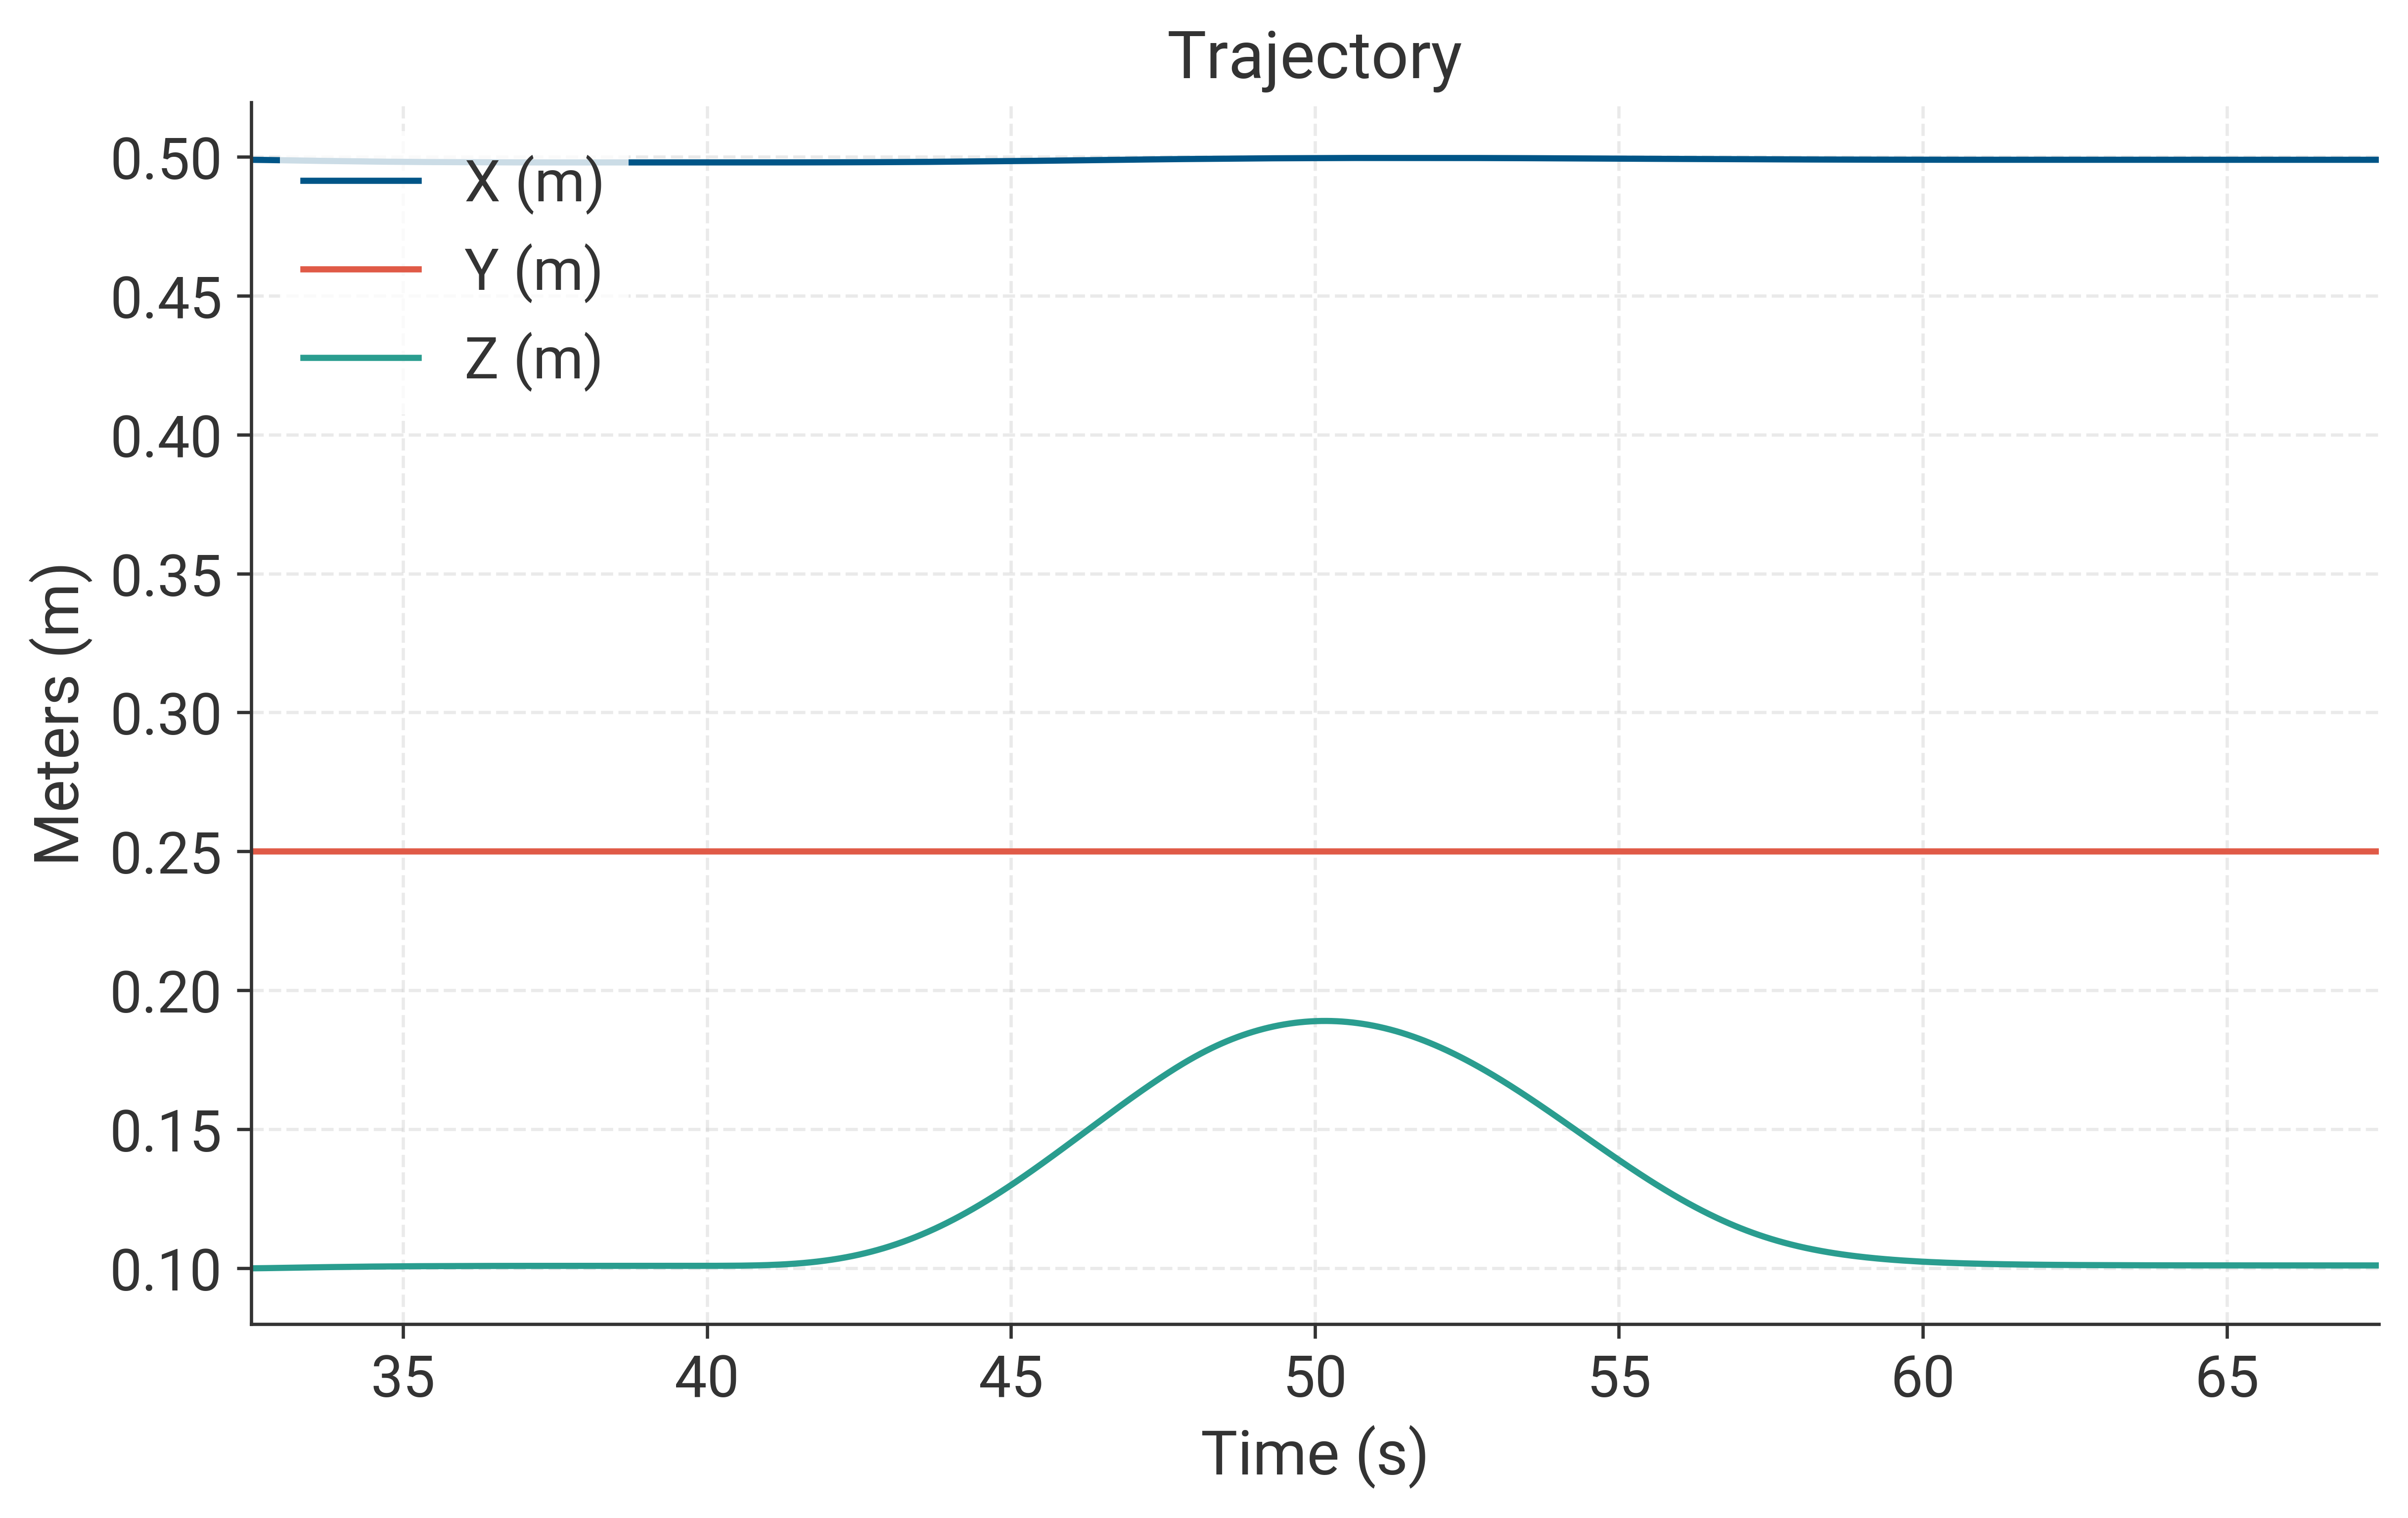
\includegraphics[width=0.85\columnwidth]{imgs/ObjectTrajecory.png}}
\caption{Kinematic results for the object. (a) Trajectory of the object, (b) velocity profile, and (c) acceleration profile during the motion.}
\label{ObjectTrajecory}
\end{figure}

\begin{figure}[htbp]
\centerline{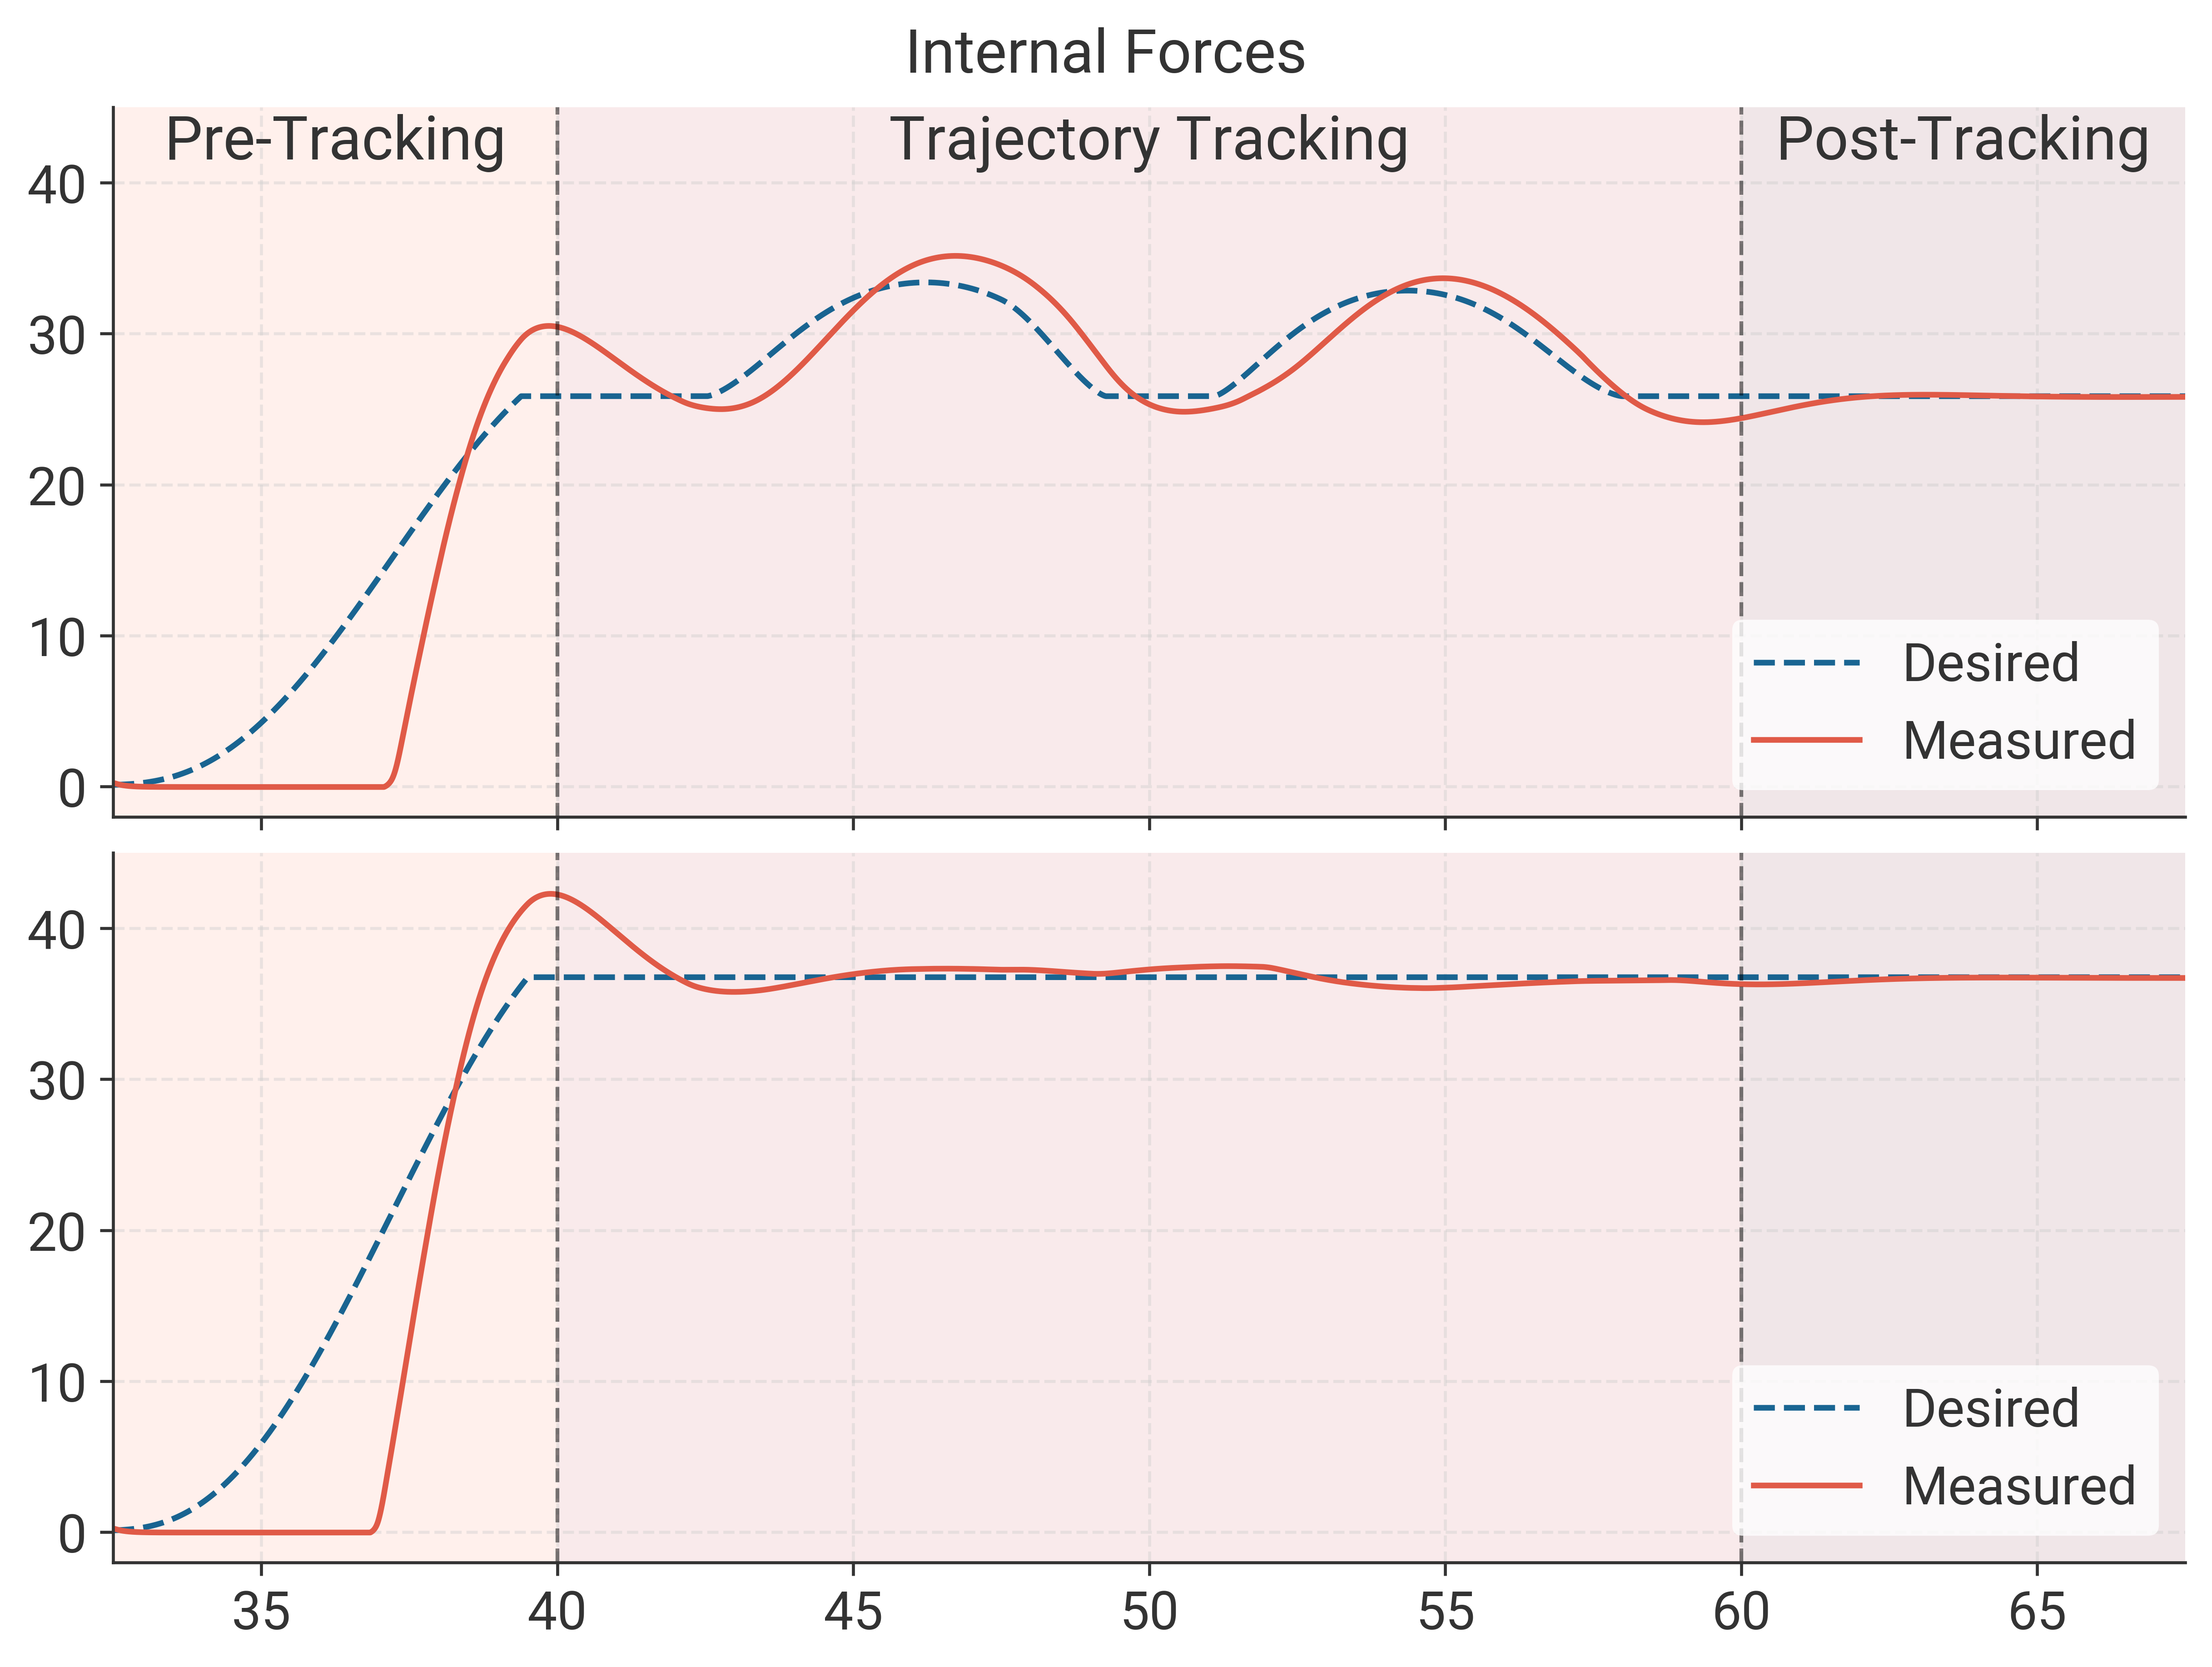
\includegraphics[width=0.85\columnwidth]{imgs/InternalForce.png}}
\caption{
 Comparison of the desired and measured internal grasping forces for two grasping strategies. 
(a) Proposed force-on-demand controller, which adaptively regulates the internal grasping force of the dual-arm system, increasing it only when required to ensure grasp stability 
(b) Baseline constant-force controller, where a fixed internal grasping force is maintained throughout the grasping task. 
The desired and measured internal forces are shown for both controllers.   
}
\label{InternalForceOnDemand}
\end{figure}

\begin{table}[htbp]
\caption{Power statistics and energy consumption for the single-cycle experiment}
\label{tab:power_statistics}
\centering
\small
\setlength{\tabcolsep}{3pt}
\begin{tabular}{|c|c|c|c|c|c|}
\hline
\textbf{Experiment} & \multicolumn{4}{c|}{\textbf{Power Statistics [W]}} & \textbf{Energy [J]} \\
\cline{2-5}
 & \textit{RMS} & \textit{Std} & \textit{Max} & \textit{Min} &  \\
\hline
Force On Demand & 12.57 & 2.81 & 15.36 & 6.11 & 428.78 \\
\hline
Constant Contact Forces & \makecell{\scriptsize(+14.9\%)} & \makecell{\scriptsize+16.6\%} & \makecell{\scriptsize+16.5\%} & \makecell{\scriptsize+8.9\%} & \makecell{\scriptsize+14.8\%} \\
\hline
\multicolumn{6}{l}{\scriptsize Values in parentheses: \% reduction relative to Force On Demand.}
\end{tabular}
\end{table}





\begin{figure}[htbp]
\centerline{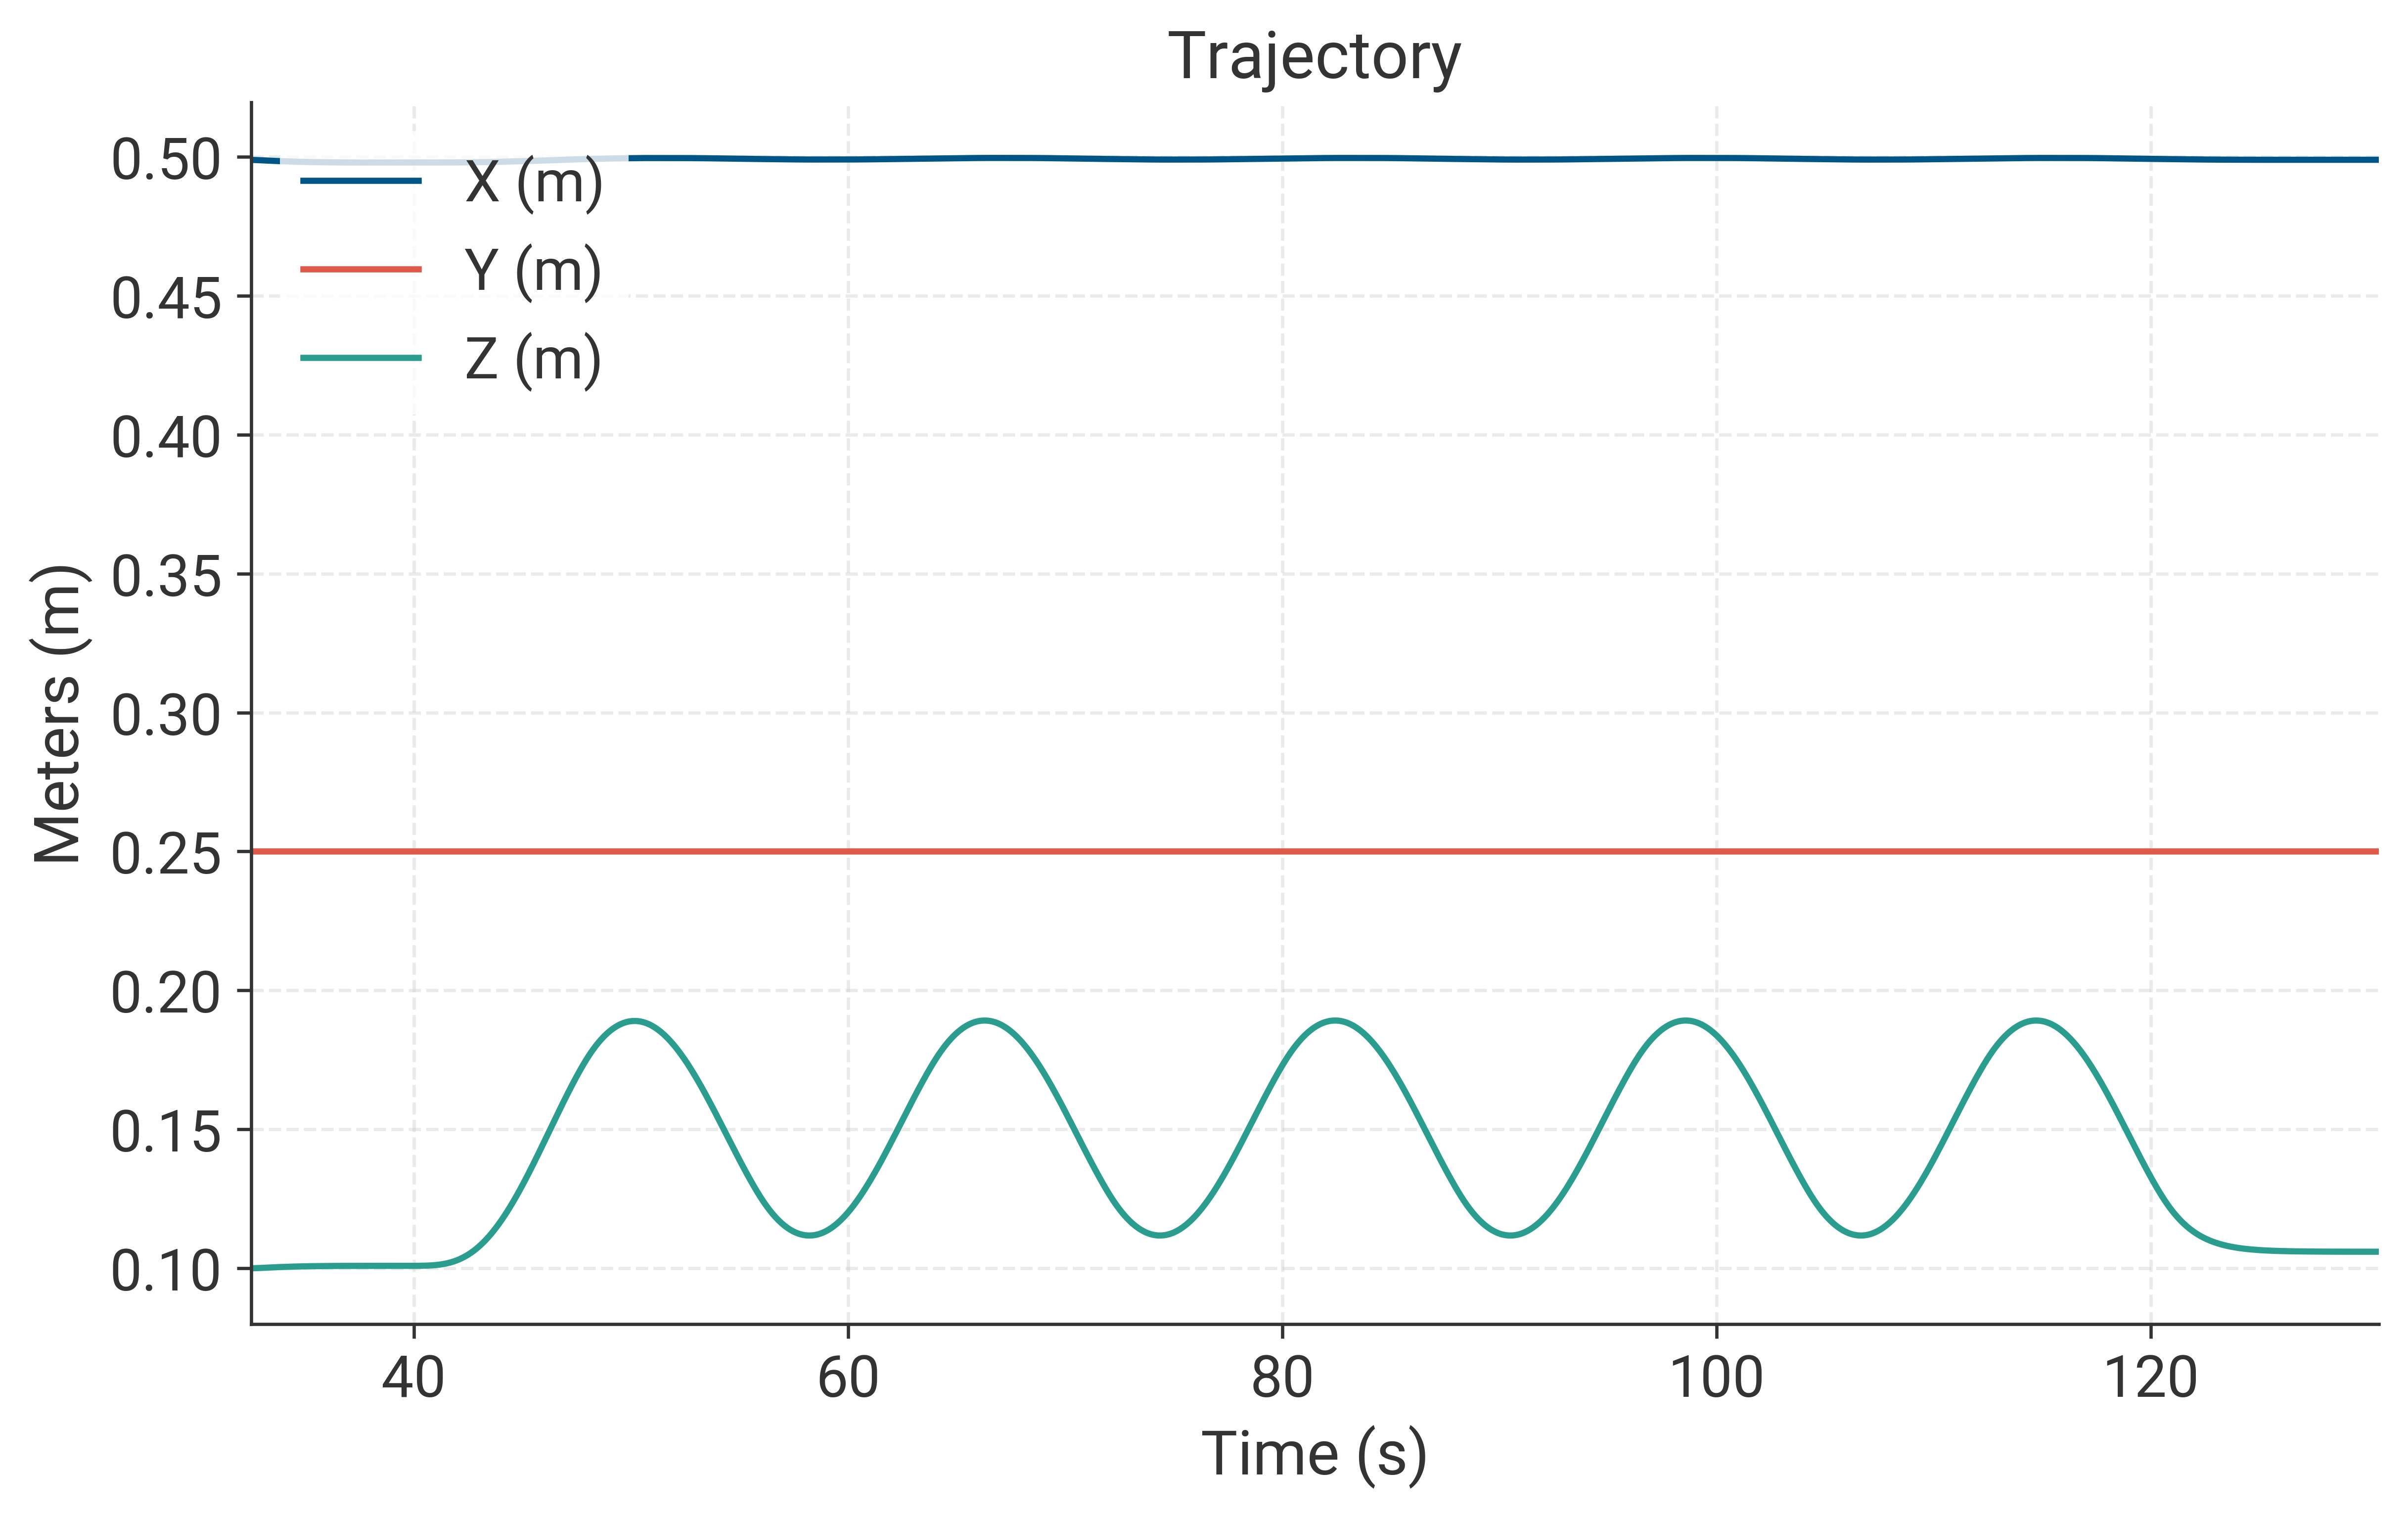
\includegraphics[width=0.85\columnwidth]{imgs/ObjectTrajecory_.png}}
\caption{Object trajectory during the cyclic waypoint-following experiment. The dual-arm system repeatedly traverses between 2 Waypoints for five consecutive cycles, demonstrating repeatable trajectory tracking.}
\label{ObjectTrajecoryFive}
\end{figure}

\begin{figure}[htbp]
\centerline{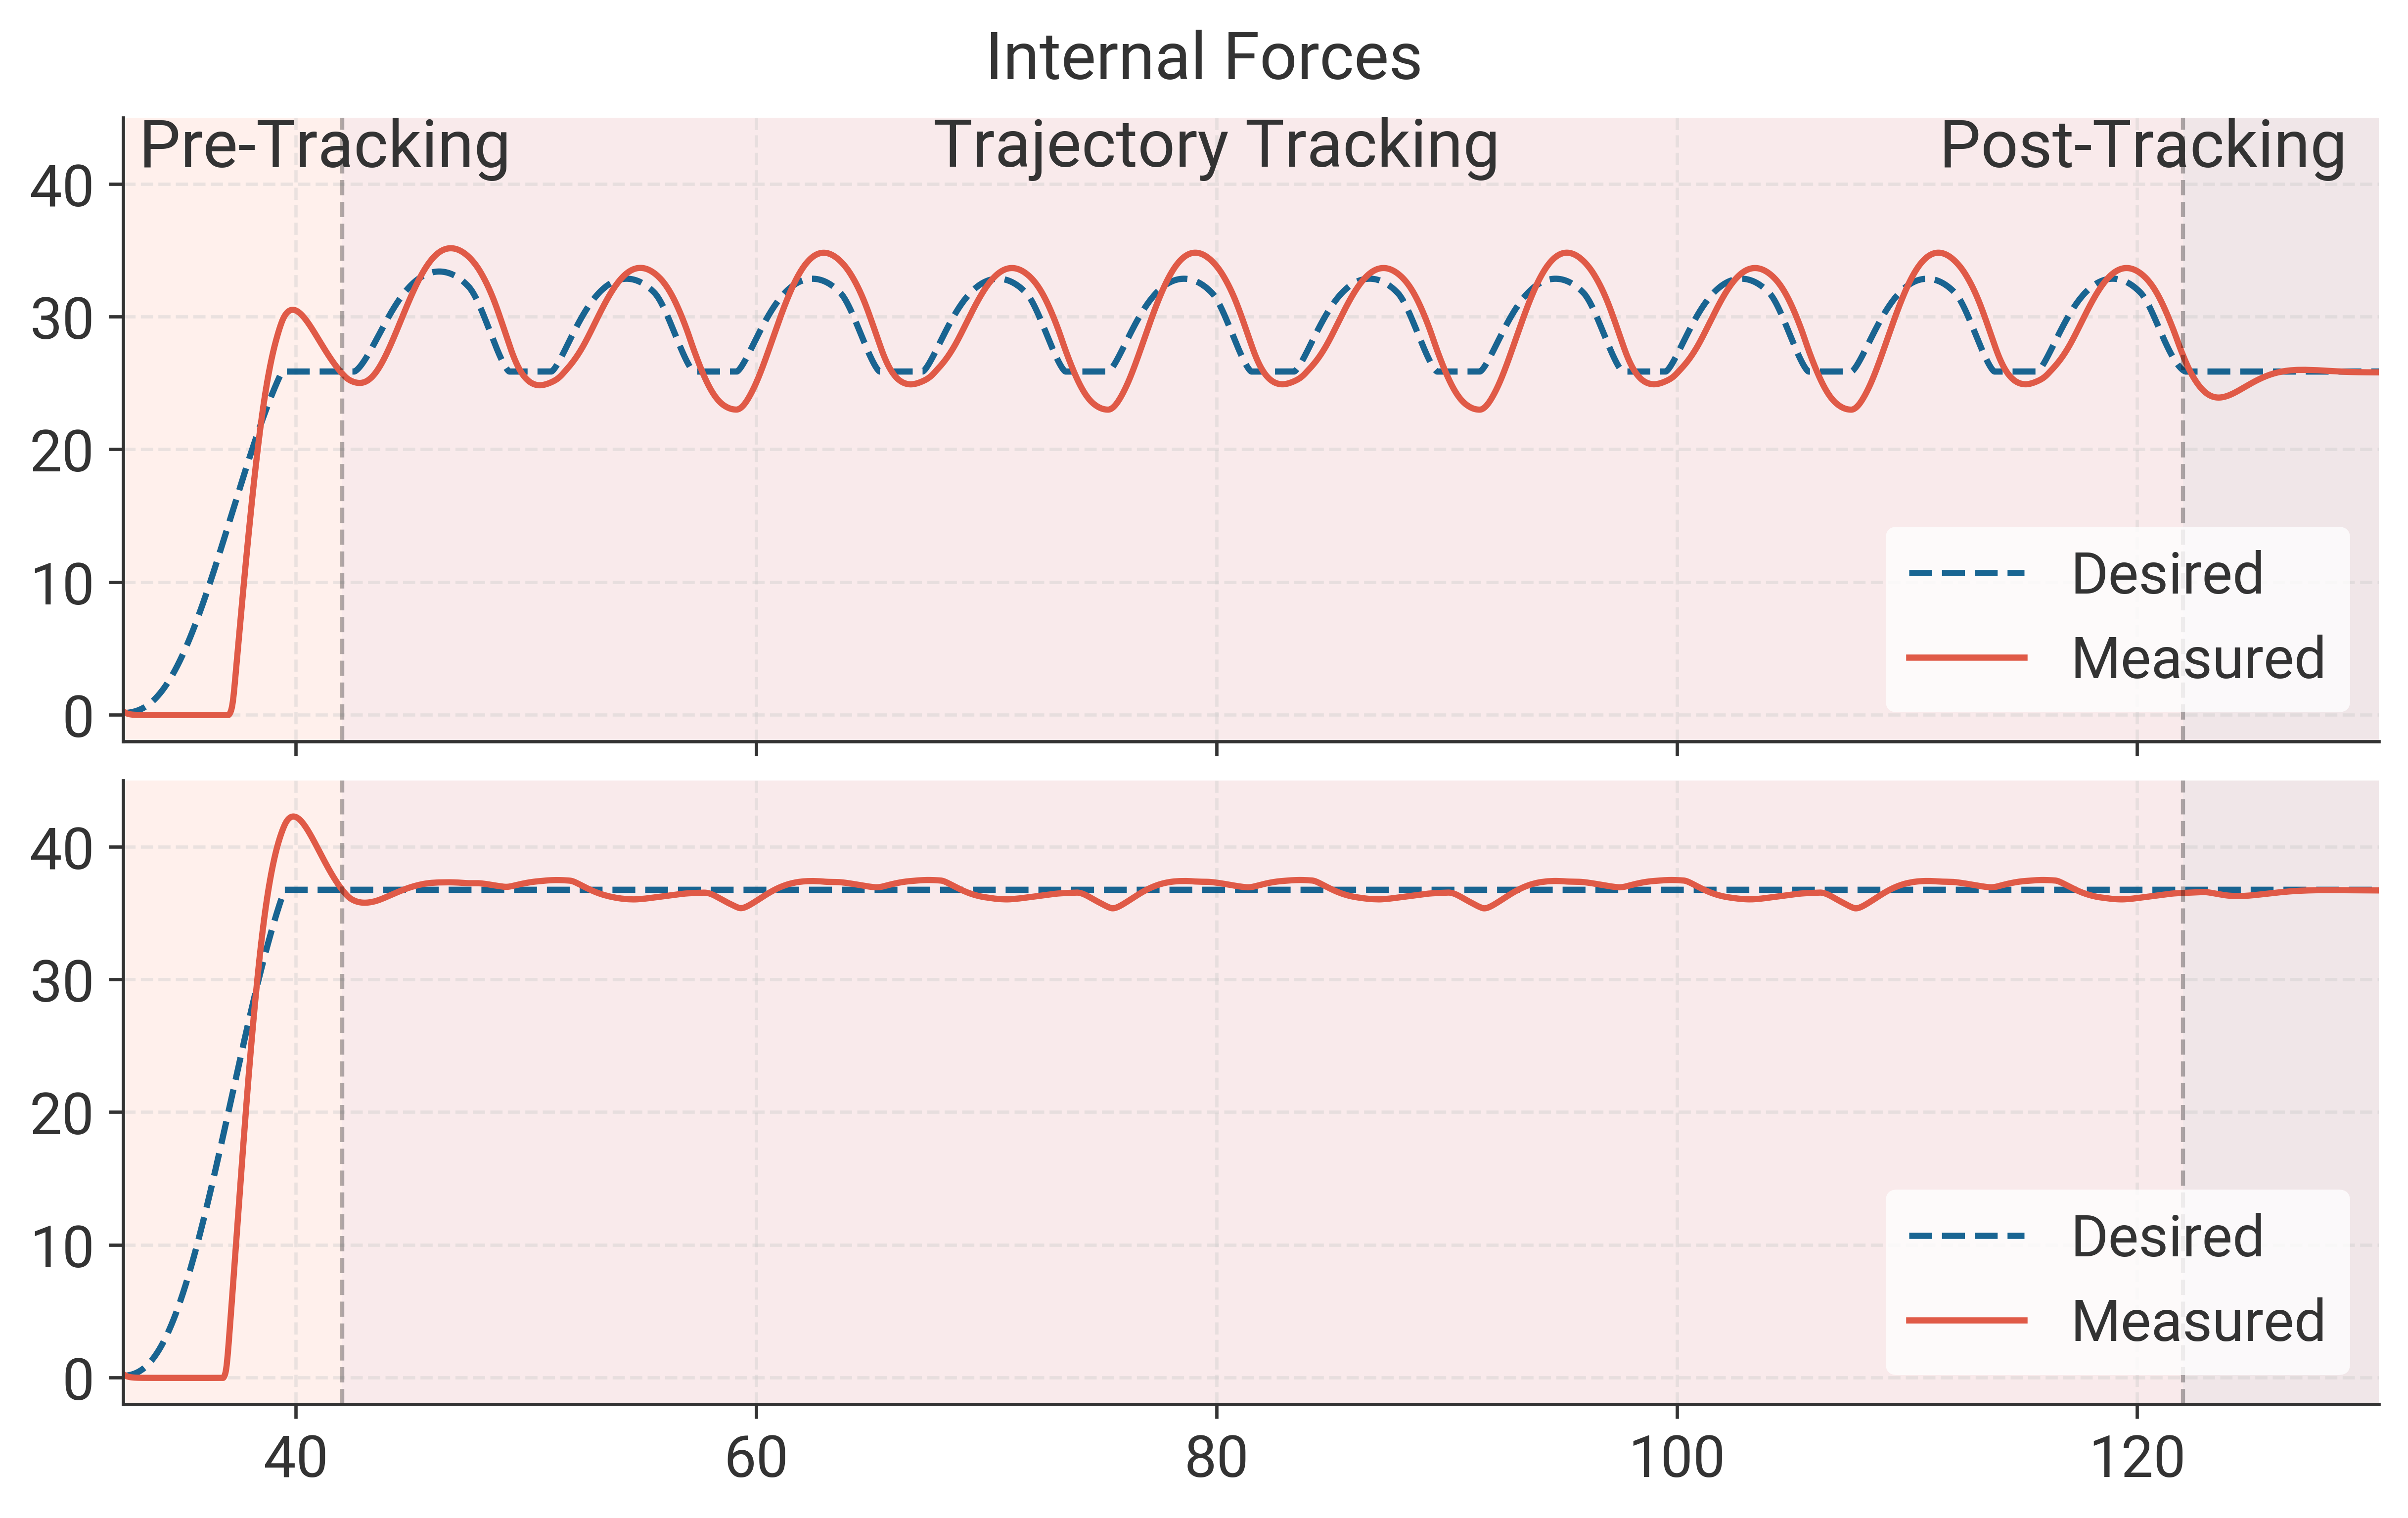
\includegraphics[width=0.85\columnwidth]{imgs/InternalForce_.png}}
\caption{Internal force tracking during the cyclic waypoint-following experiment. The dual-arm system repeatedly moves between Waypoints 1 and 2 for five consecutive cycles. (a) Proposed force-on-demand controller, which adaptively increases the internal grasping force only when necessary to enhance grasp stability. (b) Constant-force controller, which maintains a fixed internal grasping force throughout the task. The desired and measured internal forces are shown for comparison.}
\label{InternalForceOnDemandFive}
\end{figure}

\begin{table}[htbp]
\caption{Power statistics and energy consumption for the cyclic waypoint-following experiment}
\label{tab:power_statistics}
\centering
\small
\setlength{\tabcolsep}{3pt}
\begin{tabular}{|c|c|c|c|c|c|}
\hline
\textbf{Experiment} & \multicolumn{4}{c|}{\textbf{Power Statistics [W]}} & \textbf{Energy [J]} \\
\cline{2-5}
 & \textit{RMS} & \textit{Std} & \textit{Peak} & \textit{Min} &  \\
\hline
Force On Demand & 12.21 & 2.63 & 15.36 & 6.11 & 1168.53 \\
\hline
Constant Contact Forces & \makecell{14.09 \\ \scriptsize(+15.4\%)} & \makecell{2.65 \\ \scriptsize(+0.5\%)} & \makecell{17.90 \\ \scriptsize(+16.5\%)} & \makecell{6.66 \\ \scriptsize(+8.9\%)} & \makecell{1355.90 \\ \scriptsize(+16.0\%)} \\
\hline
\multicolumn{6}{l}{\scriptsize Values in parentheses: \% reduction relative to Force On Demand.}
\end{tabular}
\end{table}










\section{Discussion and Limitations}
\begin{itemize}
    \item Nonuniqueness of the internal/external decomposition: the weighted objective is a design choice, not ``the'' optimal split. State what it privileges (low effort vs.\ balance vs.\ torque margin) and how that choice was made.
    \item Linearized, one-cycle-lagged friction bound versus the exact friction cone: identify the operating regime in which this approximation may fail (e.g., fast tangential-force transients).
    \item Fixed versus state-driven weighting coefficients, \(\gamma_L\) and \(\gamma_R\): fixed weights are straightforward to justify but do not capture the instantaneous actuation capacity of each manipulator. \textbf{in future works} to present state-dependent weighting as the natural next step.
\end{itemize}
\section{Conclusion and Future Work}
\begin{itemize}
    \item \textbf{Summary:} The proposed framework combines QP-based dual-arm squeeze-force allocation, a motion-adaptive force-demand formulation, and a joint-torque-capacity-aware extension, and is validated experimentally on a dual \texttt{xArm7} platform.

    \item \textbf{Future Work:}
    \begin{itemize}
        \item Adopt the closed-loop, motion-estimated force-demand formulation as the primary approach, rather than as a fallback strategy.
        \item Replace the fixed weighting coefficients \(\gamma_L\) and \(\gamma_R\) with state-driven weights based on online measures such as manipulability, joint-torque headroom, or actuator thermal state.
        \item Incorporate exact friction-cone handling through a second-order cone programming (SOCP) formulation, subject to real-time computational constraints.
    \end{itemize}
\end{itemize}


\section{References}
\begin{itemize}
    \item \textbf{Internal force decomposition / dual-arm QP allocation}
    \begin{itemize}
        \item Nahon, M., and Angeles, J. (1992) --- QP-based minimization of internal forces in cooperating manipulators.
        \item Kwon, W., and Lee, B.H. --- NLP/QP force-distribution scheme with normal-force constraints.
        \item Recent analysis on the nonuniqueness of nonsqueezing load distributions in cooperative manipulation (2023).
        \item Admittance-QP dual-arm cobot framework regulating internal/external efforts (BAZAR, 2017--2018).
        \item Recent HQP variants for mobile/free-floating dual-arm manipulation (2025--2026).
    \end{itemize}

    \item \textbf{Grasp/contact force optimization under friction}
    \begin{itemize}
        \item Buss, M., Hashimoto, H., and Moore, J.B. (1996), \emph{Dextrous Hand Grasping Force Optimization}, IEEE Transactions on Robotics and Automation.
        \item Kerr, J., and Roth, B.; Cheng, F., and Orin, D. --- polyhedral/linear friction-cone approximations.
        \item Recent work comparing SOCP and QP formulations for real-time grasp-force control (2026).
    \end{itemize}

    \item \textbf{Motion-adaptive / slip-driven grip force}
    \begin{itemize}
        \item Westling, G., and Johansson, R.S. (1984), \emph{Factors Influencing the Force Control During Precision Grip}, Experimental Brain Research, 53:277--284.
        \item Nature Machine Intelligence (2025) --- trajectory modulation versus grip-force modulation for slip control.
        \item Human hand-acceleration modulation study for slip prevention (2024).
        \item Reactive slip control via internal-force optimization for multifingered hands (2026 arXiv).
    \end{itemize}

    \item \textbf{Joint-space capacity-aware allocation}
    \begin{itemize}
        \item Classical minimum-norm / weighted-pseudoinverse torque allocation for redundant and multi-arm systems.
        \item Whole-body and multi-contact QP controllers with torque- or actuation-margin-aware cost terms (locomotion / multi-contact force-distribution literature).
    \end{itemize}

    \item \textbf{Contact-state transition / hybrid position-force control}
    \begin{itemize}
        \item Raibert, M.H., and Craig, J.J. (1981) --- classical orthogonal position/force subspace hybrid control.
        \item Recent orthogonal interaction-frame decomposition for contact-rich manipulation (2026).
        \item Smooth controller blending / gain interpolation across contact-state transitions (changing-contact manipulation frameworks).
    \end{itemize}

    \item \textbf{Impact-aware contact establishment (background only)}
    \begin{itemize}
        \item van Steen, J.J., Coşgun, A., van de Wouw, N., and Saccon, A., \emph{Dual-Arm Impact-Aware Grasping through Time-Invariant Reference Spreading Control}, IFAC-PapersOnLine, 2023.
        \item van Steen, J.J., van den Brandt, G., van de Wouw, N., Kober, J., and Saccon, A., \emph{QP-Based Reference Spreading Control for Dual-Arm Robotic Manipulation with Planned Simultaneous Impacts}, IEEE Transactions on Robotics, 2024.
        \item Arita, H., Nakamura, H., Fujiki, T., and Tahara, K. --- \emph{Smoothly Connected Preemptive Impact Reduction and Contact Impedance Control}, 2022/2023.
        \item Khatib, O. --- effective/reflected mass in operational-space control.
        \item Wang, Y., Dehio, N., Tanguy, A., and Kheddar, A., \emph{Impact-Aware Task-Space Quadratic-Programming Control}, International Journal of Robotics Research, 2023.
    \end{itemize}
\end{itemize}

\bibliographystyle{IEEEtran}
\bibliography{references}

\end{document}


